\documentclass[usenames,dvipsnames]{beamer}

%
% Common preamble for all three parts.
%

\usetheme[block=fill]{metropolis}
\setbeamercolor{frametitle}{use=normal text, parent=normal text}

\usepackage{arevmath}
\SetSymbolFont{largesymbols}{normal}{OMX}{iwona}{m}{n}
\usepackage{fontspec}
\setmainfont{PT Sans}
\setsansfont{PT Sans}
\setmonofont{PT Mono}[Scale=0.87]
\usepackage[english,russian]{babel}
\usepackage{amsmath}
\usepackage{color}
\usepackage{minted}
\usepackage{hyperref}
\usepackage{multicol}
\usepackage{tabularx}
\usepackage{tikz}
\usepackage{tcolorbox}

% For slide 28 (Tikz examples)
\usetikzlibrary{mindmap,trees}
\usetikzlibrary{backgrounds,shapes,arrows,positioning,calc,snakes,fit}
\usepgflibrary{decorations.markings}

\hypersetup{unicode=true}

\tcbuselibrary{skins}
\tcbuselibrary{listings}
\tcbuselibrary{minted}
\tcbset{colframe=mDarkTeal, colback=white!90!mDarkTeal,% Taken from the Metropolis theme
        left=0.8em,right=0.8em}
\newtcolorbox{tblock}[1]{boxsep=1mm,sidebyside=false,bicolor=false,colback=white,title={#1}}
\newtcolorbox{printout}{boxsep=0mm,sidebyside=false,bicolor=false,colback=white}
\def\linkbox#1{\tcbox[on line,boxsep=0mm,left=2pt,right=2pt,top=2pt,bottom=2pt,
                      colback=mDarkTeal,coltext=white]{#1}}
\def\ovllink#1{\tcbox[on line,boxsep=0mm,left=2pt,right=2pt,top=2pt,bottom=2pt,
                      colback=green!30!black,colframe=green!30!black,coltext=white]{#1}}
\newtcblisting{code}{boxsep=0mm,listing only,minted language=latex}
\newtcblisting{bibtexcode}{boxsep=0mm,listing only,minted language=bibtex}
\newtcblisting{exampletwoup}{fontupper=\small,fontlower=\small,
                             boxsep=0mm,listing side text,minted language=latex,
                             bicolor,colbacklower=white,
                             righthand ratio=0.42}
\newtcblisting{exampletwouptiny}{fontupper=\footnotesize,fontlower=\footnotesize,
                                 boxsep=0mm,listing side text,minted language=latex,
                                 minted options={fontsize=\footnotesize},
                                 bicolor,colbacklower=white,
                                 righthand ratio=0.42}
\newtcblisting{exampletwouppaused}{fontupper=\footnotesize,fontlower=\footnotesize,
                             boxsep=0mm,listing side text,minted language=latex,
                             minted options={fontsize=\footnotesize},
                             bicolor,colbacklower=white,
                             righthand ratio=0.42,after lower=\onslide<1->}
\newtcbinputlisting{\inputcode}[2][]{%
listing file={#2},boxsep=0mm,listing only,minted language=latex,#1}
\newtcbinputlisting{\inputbibtexcode}[2][]{%
listing file={#2},boxsep=0mm,listing only,minted language=bibtex,#1}

% only inline todonotes work
\usepackage{xkeyval}
\usepackage[textsize=small]{todonotes}
\presetkeys{todonotes}{inline}{}

\usetikzlibrary{shapes,arrows,positioning,shadows}

% no nav buttons
\usenavigationsymbolstemplate{}

\newcommand{\bftt}[1]{\textbf{\texttt{#1}}}
%\newcommand{\comment}[1]{{\color[HTML]{008080}\textit{\textbf{\texttt{#1}}}}}
\newcommand{\cmd}[1]{{\color[HTML]{008000}\bftt{#1}}}
\newcommand{\bs}{\char`\\}
\newcommand{\cmdbs}[1]{\cmd{\bs#1}}
\newcommand{\lcb}{\char '173}
\newcommand{\rcb}{\char '175}
\newcommand{\cmdbegin}[1]{\cmdbs{begin\lcb}\bftt{#1}\cmd{\rcb}}
\newcommand{\cmdend}[1]{\cmdbs{end\lcb}\bftt{#1}\cmd{\rcb}}

\newcommand{\wllogo}{\textbf{Overleaf}}

% this is where the example source files are loaded from
% do not include a trailing slash
\newcommand{\fileuri}{https://raw.github.com/sgolovan/latex-course/master/ru}

\newcommand{\wlserver}{https://www.overleaf.com}
\newcommand{\wlnewdoc}[1]{\wlserver/docs?snip\_uri=\fileuri/#1\&splash=none}

\def\tikzname{Ti\emph{k}Z}

% from http://tex.stackexchange.com/questions/5226/keyboard-font-for-latex
\newcommand*\keystroke[1]{%
  \tikz[baseline=(key.base)]
    \node[%
      draw,
      fill=white,
      drop shadow={shadow xshift=0.25ex,shadow yshift=-0.25ex,fill=black,opacity=0.75},
      rectangle,
      rounded corners=2pt,
      inner sep=1pt,
      line width=0.5pt,
      font=\scriptsize\ttfamily
    ](key) {#1\strut}
  ;
}
\newcommand{\keystrokebftt}[1]{\keystroke{\bftt{#1}}}

% stolen from minted.dtx
\newenvironment{exampletwouptinynoframe}
  {\VerbatimEnvironment
   \begin{VerbatimOut}{example.out}}
  {\end{VerbatimOut}
   \setlength{\parindent}{0pt}
   \begin{tabular}{l|l}
   \begin{minipage}{0.55\linewidth}
     \inputminted[fontsize=\scriptsize,resetmargins]{latex}{example.out}
   \end{minipage} &
   \begin{minipage}{0.35\linewidth}
     \setlength{\parskip}{6pt plus 1pt minus 1pt}%
     \raggedright\scriptsize\input{example.out}
   \end{minipage}
   \end{tabular}}

\title{Интерактивное введение в \LaTeX}
\author{Джон Д. Лис-Миллер\\Перевод на русский язык: Сергей Головань}
%\titlegraphic{%
%\includegraphics[height=36pt]{overleaf}\\[1em]
%\includegraphics[height=24pt]{UoB-logo}
%}


\subtitle{Часть 3: Помимо статей: Презентации и не только}

\newcommand{\alice}[1]{\todo[color=green!40]{#1}}
\newcommand{\bob}[1]{\todo[color=purple!40]{#1}}

\begin{document}

%%%%%%%%%%%%%%%%%%%%%%%%%%%%%%%%%%%%%%%%%%%%%%%%%%%%%%%%%%%%%%%%%%%%%%%%%%%%%%%
%%%%%%%%%%%%%%%%%%%%%%%%%%%%%%%%%%%%%%%%%%%%%%%%%%%%%%%%%%%%%%%%%%%%%%%%%%%%%%%
%%%%%%%%%%%%%%%%%%%%%%%%%%%%%%%%%%%%%%%%%%%%%%%%%%%%%%%%%%%%%%%%%%%%%%%%%%%%%%%
\begin{frame}
\titlepage
\end{frame}

%%%%%%%%%%%%%%%%%%%%%%%%%%%%%%%%%%%%%%%%%%%%%%%%%%%%%%%%%%%%%%%%%%%%%%%%%%%%%%%
%%%%%%%%%%%%%%%%%%%%%%%%%%%%%%%%%%%%%%%%%%%%%%%%%%%%%%%%%%%%%%%%%%%%%%%%%%%%%%%
%%%%%%%%%%%%%%%%%%%%%%%%%%%%%%%%%%%%%%%%%%%%%%%%%%%%%%%%%%%%%%%%%%%%%%%%%%%%%%%
%\begin{frame}{Setup}
%\begin{itemize}
%\item Go to this URL in Google Chrome (\emph{not} Internet Explorer) to open
%these slides on your computer:
%\vskip 2em
%\begin{center}
%\fbox{\url{http://bit.ly/12WWWqj}}
%\end{center}
%\vskip 2em
%\item Here are the slides from the previous tutorial, for reference:
%\begin{center}
%\vskip 1em
%\fbox{\href{https://dl.dropboxusercontent.com/u/31383671/site/latex_course_v2/part1.pdf}{Part 1: The Basics}}
%\vskip 1em
%\fbox{\href{https://dl.dropboxusercontent.com/u/31383671/site/latex_course_v2/part2.pdf}{Part 2: Structured Documents \& More}}
%\end{center}
%\end{itemize}
%\end{frame}

%%%%%%%%%%%%%%%%%%%%%%%%%%%%%%%%%%%%%%%%%%%%%%%%%%%%%%%%%%%%%%%%%%%%%%%%%%%%%%%
%%%%%%%%%%%%%%%%%%%%%%%%%%%%%%%%%%%%%%%%%%%%%%%%%%%%%%%%%%%%%%%%%%%%%%%%%%%%%%%
%%%%%%%%%%%%%%%%%%%%%%%%%%%%%%%%%%%%%%%%%%%%%%%%%%%%%%%%%%%%%%%%%%%%%%%%%%%%%%%
\section{\LaTeX{}, повторение}

%%%%%%%%%%%%%%%%%%%%%%%%%%%%%%%%%%%%%%%%%%%%%%%%%%%%%%%%%%%%%%%%%%%%%%%%%%%%%%%
%%%%%%%%%%%%%%%%%%%%%%%%%%%%%%%%%%%%%%%%%%%%%%%%%%%%%%%%%%%%%%%%%%%%%%%%%%%%%%%
%%%%%%%%%%%%%%%%%%%%%%%%%%%%%%%%%%%%%%%%%%%%%%%%%%%%%%%%%%%%%%%%%%%%%%%%%%%%%%%
\begin{frame}[fragile]{\insertsection}
\begin{itemize}
\item Вы набираете документ в формате \emph{обычного текста} с \cmd{командами},
  которые описывают его структуру и смысл.
\item Программа \texttt{latex} обрабатывает ваш текст и команды и преобразовывает
  его в красиво отформатированный документ.
\end{itemize}
\begin{center}
\begin{code}
Шла Саша по шоссе и сосала \emph{сушку}.
\end{code}
\tikz\node[single arrow,fill=gray,font=\ttfamily\bfseries,%
  rotate=270,xshift=-1em]{latex};
\begin{printout}
Шла Саша по шоссе и сосала \emph{сушку}.
\end{printout}
\end{center}
\end{frame}

%%%%%%%%%%%%%%%%%%%%%%%%%%%%%%%%%%%%%%%%%%%%%%%%%%%%%%%%%%%%%%%%%%%%%%%%%%%%%%%
%%%%%%%%%%%%%%%%%%%%%%%%%%%%%%%%%%%%%%%%%%%%%%%%%%%%%%%%%%%%%%%%%%%%%%%%%%%%%%%
%%%%%%%%%%%%%%%%%%%%%%%%%%%%%%%%%%%%%%%%%%%%%%%%%%%%%%%%%%%%%%%%%%%%%%%%%%%%%%%
\begin{frame}[fragile]{\insertsection: Команды и аргументы}
\begin{itemize}
\item Команды начинаются с \emph{обратной косой} \keystrokebftt{\bs}.
\item Некоторые команды принимают \emph{аргументы} в фигурных скобках \keystrokebftt{\{}
\keystrokebftt{\}}.
\item Некоторые команды также принимают \emph{необязательные аргументы} в
  квадратных скобках \keystrokebftt{[} \keystrokebftt{]}.
\vskip 2ex
\begin{exampletwouptiny}
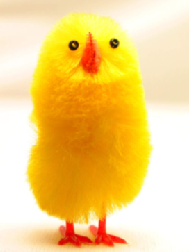
\includegraphics[
width=0.5\textwidth]{big_chick}

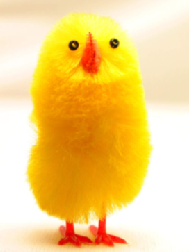
\includegraphics[
width=0.3\textwidth,
angle=270]{big_chick}
\end{exampletwouptiny}
\end{itemize}
\end{frame}

%%%%%%%%%%%%%%%%%%%%%%%%%%%%%%%%%%%%%%%%%%%%%%%%%%%%%%%%%%%%%%%%%%%%%%%%%%%%%%%
%%%%%%%%%%%%%%%%%%%%%%%%%%%%%%%%%%%%%%%%%%%%%%%%%%%%%%%%%%%%%%%%%%%%%%%%%%%%%%%
%%%%%%%%%%%%%%%%%%%%%%%%%%%%%%%%%%%%%%%%%%%%%%%%%%%%%%%%%%%%%%%%%%%%%%%%%%%%%%%
\begin{frame}[fragile]{\insertsection: Окружения}
\begin{itemize}
\item Команды \cmdbs{begin} и \cmdbs{end} применяются, чтобы создавать много
  разных окружений --- контекстов.

\item Окружения \bftt{itemize} и \bftt{enumerate} печатают списки.
\vskip 2ex
\begin{exampletwouptiny}
% ненумерованный список
\begin{itemize}
\item Печенье
\item Чай
\end{itemize}

%нумерованный список
\begin{enumerate}
\item Печенье
\item Чай
\end{enumerate}
\end{exampletwouptiny}
\end{itemize}
\end{frame}

%%%%%%%%%%%%%%%%%%%%%%%%%%%%%%%%%%%%%%%%%%%%%%%%%%%%%%%%%%%%%%%%%%%%%%%%%%%%%%%
%%%%%%%%%%%%%%%%%%%%%%%%%%%%%%%%%%%%%%%%%%%%%%%%%%%%%%%%%%%%%%%%%%%%%%%%%%%%%%%
%%%%%%%%%%%%%%%%%%%%%%%%%%%%%%%%%%%%%%%%%%%%%%%%%%%%%%%%%%%%%%%%%%%%%%%%%%%%%%%
\begin{frame}[fragile]{\insertsection: Набор математики}
\vspace{-3ex}
\small
\begin{itemize}
\item Окружение \bftt{equation} создаёт пронумерованное уравнение.
\begin{exampletwouptiny}
\begin{equation}
  \sum_{k=1}^{n} \frac{1}{2^k}
\end{equation}
\end{exampletwouptiny}
\item Значки доллара \keystrokebftt{\$} применяются для математики в тексте.
\begin{exampletwouptiny}
% результат так себе:
Пусть a и b --- два разных
натуральных числа и пусть
c = a - b + 1.

% так намного лучше:
Пусть $a$ и $b$ --- два разных
натуральных числа и пусть
$c = a - b + 1$.
\end{exampletwouptiny}
\item Первый значок начинает формулу, второй заканчивает.\\
{\scriptsize Но можно было бы писать \bftt{\$...\$} как
\cmdbegin{math}\bftt{...}\cmdend{math}.}
\end{itemize}
\end{frame}

%%%%%%%%%%%%%%%%%%%%%%%%%%%%%%%%%%%%%%%%%%%%%%%%%%%%%%%%%%%%%%%%%%%%%%%%%%%%%%%
%%%%%%%%%%%%%%%%%%%%%%%%%%%%%%%%%%%%%%%%%%%%%%%%%%%%%%%%%%%%%%%%%%%%%%%%%%%%%%%
%%%%%%%%%%%%%%%%%%%%%%%%%%%%%%%%%%%%%%%%%%%%%%%%%%%%%%%%%%%%%%%%%%%%%%%%%%%%%%%
\begin{frame}[fragile]{\insertsection: Структура документа}
\vspace{-3ex}
\begin{itemize}{\small
\item Начинается с команды \cmdbs{documentclass} --- тип документа.
\item Метаинформация (\cmdbs{title} и \cmdbs{author}) и список пакетов в преамбуле.
\item Содержимое между \cmdbegin{document} и \cmdend{document}.
\item Команда \cmdbs{maketitle} создаёт название; команы \cmdbs{section}
формируют пронумерованные разделы.
}\end{itemize}
\vspace{-4ex}
\begin{minipage}{0.55\linewidth}
\inputcode[minted options={fontsize=\footnotesize}]{recap-structure.tex}
\end{minipage}~~%
\begin{minipage}{0.45\linewidth}
\includegraphics[width=\textwidth,clip,viewport=0cm 227mm 5cm 297mm]{recap-structure.pdf}
\end{minipage}
\end{frame}

%%%%%%%%%%%%%%%%%%%%%%%%%%%%%%%%%%%%%%%%%%%%%%%%%%%%%%%%%%%%%%%%%%%%%%%%%%%%%%%
%%%%%%%%%%%%%%%%%%%%%%%%%%%%%%%%%%%%%%%%%%%%%%%%%%%%%%%%%%%%%%%%%%%%%%%%%%%%%%%
%%%%%%%%%%%%%%%%%%%%%%%%%%%%%%%%%%%%%%%%%%%%%%%%%%%%%%%%%%%%%%%%%%%%%%%%%%%%%%%
\begin{frame}[fragile]{\insertsection: Упражнение}
\vspace{-3ex}
\begin{enumerate}
\item Вот текст небольшой статьи:\footnote{Основана на \url{http://www.cgd.ucar.edu/cms/agu/scientific_talk.html}}
\begin{center}
\ovllink{\href{\wlnewdoc{recap-exercise.tex}}{%
Щёлкните, чтобы открыть упражнение в \wllogo{}}}
\end{center}
\item Вставьте в него команды \LaTeX{} и сделайте, чтобы он выглядел как этот:
\begin{center}
\linkbox{\href{\fileuri/recap-exercise-solution.pdf}, \emph{экранируйте} его обратной косой (\cmdbs{\%}).
\item Чтобы вывести уравнение, используйте \cmdbs{frac} для дроби и команды
  \cmdbs{left(} и \cmdbs{right)} для скобок.
\end{itemize}
\end{tblock}
\vspace{5pt}
\end{frame}

%%%%%%%%%%%%%%%%%%%%%%%%%%%%%%%%%%%%%%%%%%%%%%%%%%%%%%%%%%%%%%%%%%%%%%%%%%%%%%%
%%%%%%%%%%%%%%%%%%%%%%%%%%%%%%%%%%%%%%%%%%%%%%%%%%%%%%%%%%%%%%%%%%%%%%%%%%%%%%%
%%%%%%%%%%%%%%%%%%%%%%%%%%%%%%%%%%%%%%%%%%%%%%%%%%%%%%%%%%%%%%%%%%%%%%%%%%%%%%%
\section{Презентации в \protect\bftt{beamer}}

%%%%%%%%%%%%%%%%%%%%%%%%%%%%%%%%%%%%%%%%%%%%%%%%%%%%%%%%%%%%%%%%%%%%%%%%%%%%%%%
%%%%%%%%%%%%%%%%%%%%%%%%%%%%%%%%%%%%%%%%%%%%%%%%%%%%%%%%%%%%%%%%%%%%%%%%%%%%%%%
%%%%%%%%%%%%%%%%%%%%%%%%%%%%%%%%%%%%%%%%%%%%%%%%%%%%%%%%%%%%%%%%%%%%%%%%%%%%%%%
\begin{frame}[fragile]{\insertsection}
\vspace{-1ex}
\begin{itemize}
  \item Beamer это пакет для создания презентаций (таких как эта, кстати!) в
\LaTeX{}.
\item Он предоставляет класс документа \bftt{beamer}.
\item Окружение \bftt{frame} применяется для создания слайдов.
\end{itemize}
\begin{minipage}{0.55\linewidth}
\inputcode[minted options={fontsize=\scriptsize}]{beamer-minimal.tex}
\end{minipage}~~%
\begin{minipage}{0.5\linewidth}
% trim: l b r t
\includegraphics[width=\textwidth,clip,trim=1.33in 1in 1.33in 1in]{beamer-minimal.pdf}
\end{minipage}
\end{frame}

%%%%%%%%%%%%%%%%%%%%%%%%%%%%%%%%%%%%%%%%%%%%%%%%%%%%%%%%%%%%%%%%%%%%%%%%%%%%%%%
%%%%%%%%%%%%%%%%%%%%%%%%%%%%%%%%%%%%%%%%%%%%%%%%%%%%%%%%%%%%%%%%%%%%%%%%%%%%%%%
%%%%%%%%%%%%%%%%%%%%%%%%%%%%%%%%%%%%%%%%%%%%%%%%%%%%%%%%%%%%%%%%%%%%%%%%%%%%%%%
\begin{frame}[fragile]{\insertsection: Следование примерам}

\begin{itemize}
\item Пока мы будем проходить следующие слайды, пробуйте примеры из них, набирая
  их в примере документа в \wllogo.
\end{itemize}
\vskip 2ex
\begin{center}
\ovllink{\href{\wlnewdoc{beamer-minimal.tex}}{%
Щёлкните, чтобы открыть пример документа в \wllogo{}}}
\end{center}
\end{frame}

%%%%%%%%%%%%%%%%%%%%%%%%%%%%%%%%%%%%%%%%%%%%%%%%%%%%%%%%%%%%%%%%%%%%%%%%%%%%%%%
%%%%%%%%%%%%%%%%%%%%%%%%%%%%%%%%%%%%%%%%%%%%%%%%%%%%%%%%%%%%%%%%%%%%%%%%%%%%%%%
%%%%%%%%%%%%%%%%%%%%%%%%%%%%%%%%%%%%%%%%%%%%%%%%%%%%%%%%%%%%%%%%%%%%%%%%%%%%%%%
\begin{frame}[fragile]
\frametitle{\insertsection: Фреймы}
\begin{itemize}
\item Используйте команду \cmdbs{frametitle}, чтобы задать название фрейму.
\item Потом добавьте содержимое фрейма.
\item Исходный код фрейма выглядит примерно так:
\vskip 2ex
\inputcode[minted options={fontsize=\scriptsize}]{beamer-frame.tex}
\end{itemize}
\end{frame}

%%%%%%%%%%%%%%%%%%%%%%%%%%%%%%%%%%%%%%%%%%%%%%%%%%%%%%%%%%%%%%%%%%%%%%%%%%%%%%%
%%%%%%%%%%%%%%%%%%%%%%%%%%%%%%%%%%%%%%%%%%%%%%%%%%%%%%%%%%%%%%%%%%%%%%%%%%%%%%%
%%%%%%%%%%%%%%%%%%%%%%%%%%%%%%%%%%%%%%%%%%%%%%%%%%%%%%%%%%%%%%%%%%%%%%%%%%%%%%%
\begin{frame}[fragile]{\insertsection: Разделы}
\begin{itemize}
\item Можно применять команды \cmdbs{section}, чтобы группировать \bftt{frame}ы,
и \bftt{beamer} использует их ддя автоматического создания плана.
\item Чтобы сгенерировать план, используйте команду \cmdbs{tableofcontents}.
Вот как она выглядит для текущей презентации. Необязательный аргумент
\bftt{currentsection} выделяет текущий раздел.
\vskip 2ex
\begin{exampletwouptiny}
\tableofcontents[currentsection]
\end{exampletwouptiny}
\end{itemize}
\end{frame}

%%%%%%%%%%%%%%%%%%%%%%%%%%%%%%%%%%%%%%%%%%%%%%%%%%%%%%%%%%%%%%%%%%%%%%%%%%%%%%%
%%%%%%%%%%%%%%%%%%%%%%%%%%%%%%%%%%%%%%%%%%%%%%%%%%%%%%%%%%%%%%%%%%%%%%%%%%%%%%%
%%%%%%%%%%%%%%%%%%%%%%%%%%%%%%%%%%%%%%%%%%%%%%%%%%%%%%%%%%%%%%%%%%%%%%%%%%%%%%%
\begin{frame}[fragile]{\insertsection: Несколько колонок}
\begin{columns}
\begin{column}{0.4\textwidth}
\begin{itemize}
\item Окружения \bftt{columns} и \bftt{column} позволяют разбить слайд на
  несколько колонок.
\item Аргумент окружения \bftt{column} задаёт ширину колонки.
\item Также можно посмотреть на пакет \bftt{multicol}, он автоматически разбивает
  текст на несколько колонок.
\end{itemize}
\end{column}
\begin{column}{0.6\textwidth}
\begin{code}
\begin{columns}
  \begin{column}{0.4\textwidth}
    \begin{itemize}
    \item Окружения ...
    \item Аргумент окружения ...
    \item Также можно ...
    \end{itemize}
  \end{column}
  \begin{column}{0.6\textwidth}
    % вторая колонка
  \end{column}
\end{columns}
\end{code}
\end{column}
\end{columns}
\end{frame}

%%%%%%%%%%%%%%%%%%%%%%%%%%%%%%%%%%%%%%%%%%%%%%%%%%%%%%%%%%%%%%%%%%%%%%%%%%%%%%%
%%%%%%%%%%%%%%%%%%%%%%%%%%%%%%%%%%%%%%%%%%%%%%%%%%%%%%%%%%%%%%%%%%%%%%%%%%%%%%%
%%%%%%%%%%%%%%%%%%%%%%%%%%%%%%%%%%%%%%%%%%%%%%%%%%%%%%%%%%%%%%%%%%%%%%%%%%%%%%%
\begin{frame}[fragile]{\insertsection: Выделение}
\begin{itemize}

\item Используйте \cmdbs{emph} или \cmdbs{alert}, чтобы выделить текст:
\vskip 1ex
\begin{exampletwouptiny}
Я хочу \emph{подчеркнуть}, что
это очень \alert{важная} точка.
\end{exampletwouptiny}
\vskip 1ex

\item Или просто укажите, что текст жирный или курсивный:
\vskip 1ex
\begin{exampletwouptiny}
Текст \textbf{жирным} шрифтом.
Текст набран \textit{курсивом}.
\end{exampletwouptiny}
\vskip 1ex

\item Или же укажите цвет непосредственно (по-английски):
\vskip 1ex
\begin{exampletwouptiny}
Она \textcolor{red}{тормозит}
и \textcolor{green}{ускоряется}.
\end{exampletwouptiny}
\vskip 1ex
\item Смотрите \url{http://www.math.umbc.edu/~rouben/beamer/quickstart-Z-H-25.html},
и найдёте ещё цвета.
\end{itemize}
\end{frame}

%%%%%%%%%%%%%%%%%%%%%%%%%%%%%%%%%%%%%%%%%%%%%%%%%%%%%%%%%%%%%%%%%%%%%%%%%%%%%%%
%%%%%%%%%%%%%%%%%%%%%%%%%%%%%%%%%%%%%%%%%%%%%%%%%%%%%%%%%%%%%%%%%%%%%%%%%%%%%%%
%%%%%%%%%%%%%%%%%%%%%%%%%%%%%%%%%%%%%%%%%%%%%%%%%%%%%%%%%%%%%%%%%%%%%%%%%%%%%%%
\begin{frame}[fragile]{\insertsection: Иллюстрации}
\begin{itemize}
\item Используйте \cmdbs{includegraphics} из пакета \bftt{graphicx}.
\item Окружение \bftt{figure} в \bftt{beamer} по умолчанию центрирует.
\vskip 2ex
\begin{exampletwouptiny}
\begin{figure}
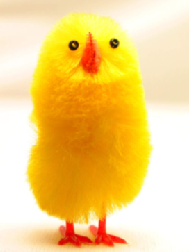
\includegraphics[
 width=0.5\textwidth]{big_chick}
\end{figure}
\end{exampletwouptiny}
\end{itemize}
\end{frame}

%%%%%%%%%%%%%%%%%%%%%%%%%%%%%%%%%%%%%%%%%%%%%%%%%%%%%%%%%%%%%%%%%%%%%%%%%%%%%%%
%%%%%%%%%%%%%%%%%%%%%%%%%%%%%%%%%%%%%%%%%%%%%%%%%%%%%%%%%%%%%%%%%%%%%%%%%%%%%%%
%%%%%%%%%%%%%%%%%%%%%%%%%%%%%%%%%%%%%%%%%%%%%%%%%%%%%%%%%%%%%%%%%%%%%%%%%%%%%%%
\begin{frame}[fragile]{\insertsection: Таблицы}
\vspace{-3ex}
\begin{itemize}\small
\item Чтобы привыкнуть к таблицам в \LaTeX{}, нужно время.
\item Можно воспользоваться окружением \bftt{tabular}.
\item Аргумент задаёт выравнивание колонок --- \textbf{l}eft, \textbf{r}ight, \textbf{r}ight.
\begin{exampletwouptiny}
\begin{tabular}{lrr}
Прод.  & \# & Цена \$ \\
Гаджет & 1  & 199.99  \\
Виджет & 2  & 399.99  \\
\end{tabular}
\end{exampletwouptiny}
\vspace{-1ex}
\item В нём также задаются вертикальные линии; команда \cmdbs{hline} проводит горизонтальную линию.
\begin{exampletwouptiny}
\begin{tabular}{|l|r|r|} \hline
Прод.  & \# & Цена \$ \\\hline
Виджет & 1  & 199.99  \\
Гаджет & 2  & 399.99  \\\hline
\end{tabular}
\end{exampletwouptiny}
\item Амперсанд \keystrokebftt{\&} разделяет колонки, а двойная обратная косая
  \keystrokebftt{\bs}\keystrokebftt{\bs} начинает новую строку.
\end{itemize}
\end{frame}

%%%%%%%%%%%%%%%%%%%%%%%%%%%%%%%%%%%%%%%%%%%%%%%%%%%%%%%%%%%%%%%%%%%%%%%%%%%%%%%
%%%%%%%%%%%%%%%%%%%%%%%%%%%%%%%%%%%%%%%%%%%%%%%%%%%%%%%%%%%%%%%%%%%%%%%%%%%%%%%
%%%%%%%%%%%%%%%%%%%%%%%%%%%%%%%%%%%%%%%%%%%%%%%%%%%%%%%%%%%%%%%%%%%%%%%%%%%%%%%
\begin{frame}[fragile]{\insertsection: Блоки}
\begin{itemize}
\item Окружение \bftt{block} создаёт озаглавленный блок.
\begin{exampletwouptiny}
\begin{block}{Интересный факт}
Это очень важно.
\end{block}

\begin{alertblock}{Предупреждаю}
Это действительно очень важно!
\end{alertblock}
\end{exampletwouptiny}

\item Как на самом деле выглядит блок, зависит от темы оформления\dots
\end{itemize}
\end{frame}

%%%%%%%%%%%%%%%%%%%%%%%%%%%%%%%%%%%%%%%%%%%%%%%%%%%%%%%%%%%%%%%%%%%%%%%%%%%%%%%
%%%%%%%%%%%%%%%%%%%%%%%%%%%%%%%%%%%%%%%%%%%%%%%%%%%%%%%%%%%%%%%%%%%%%%%%%%%%%%%
%%%%%%%%%%%%%%%%%%%%%%%%%%%%%%%%%%%%%%%%%%%%%%%%%%%%%%%%%%%%%%%%%%%%%%%%%%%%%%%
\begin{frame}[fragile]
\frametitle{\insertsection: Темы оформления}
\vspace{-3ex}
\begin{itemize}
\item Выбирайте, как выглядит презентация, с помощью тем оформления.
\item Смотрите \url{http://deic.uab.es/~iblanes/beamer_gallery/index_by_theme.html}
и найдёте там большую коллекцию тем.
\end{itemize}
\begin{minipage}{0.56\linewidth}
\inputcode[minted options={fontsize=\scriptsize}]{beamer-theme.tex}
\end{minipage}~~%
\begin{minipage}{0.5\linewidth}
% trim: l b r t
\includegraphics[width=\textwidth,clip,trim=0.67in 1.18in 2in 0.82in]{beamer-theme.pdf}
\end{minipage}
\end{frame}

%%%%%%%%%%%%%%%%%%%%%%%%%%%%%%%%%%%%%%%%%%%%%%%%%%%%%%%%%%%%%%%%%%%%%%%%%%%%%%%
%%%%%%%%%%%%%%%%%%%%%%%%%%%%%%%%%%%%%%%%%%%%%%%%%%%%%%%%%%%%%%%%%%%%%%%%%%%%%%%
%%%%%%%%%%%%%%%%%%%%%%%%%%%%%%%%%%%%%%%%%%%%%%%%%%%%%%%%%%%%%%%%%%%%%%%%%%%%%%%
\begin{frame}[fragile]
\frametitle{\insertsection: Анимация}
\begin{itemize}
\item Один фрейм может генерировать несколько слайдов.
\item Применяйте команду \cmdbs{pause}, чтобы показать только часть слайда.
\vskip 2ex
\begin{exampletwouppaused}
\begin{itemize}
\item Чувствуете
\pause \item предвкушение?
\end{itemize}
\end{exampletwouppaused}
\vskip 2ex
\item<2-> Существует много более гибких способов создавать анимацию в \bftt{beamer};
смотрите также команды \cmdbs{only}, \cmdbs{alt} и \cmdbs{uncover}.
\end{itemize}
\end{frame}

%%%%%%%%%%%%%%%%%%%%%%%%%%%%%%%%%%%%%%%%%%%%%%%%%%%%%%%%%%%%%%%%%%%%%%%%%%%%%%%
%%%%%%%%%%%%%%%%%%%%%%%%%%%%%%%%%%%%%%%%%%%%%%%%%%%%%%%%%%%%%%%%%%%%%%%%%%%%%%%
%%%%%%%%%%%%%%%%%%%%%%%%%%%%%%%%%%%%%%%%%%%%%%%%%%%%%%%%%%%%%%%%%%%%%%%%%%%%%%%
\begin{frame}[fragile]
\frametitle{\insertsection: Упражнение}
Воссоздайте прекрасную <<Презентацию о Геттисберге>> Питера Норвига в
\bftt{beamer}.\footnote{\url{http://norvig.com/Gettysburg}}

\begin{enumerate}
\item Откройте это упражнение в \wllogo{}:
\begin{printout}
\href{\wlnewdoc{beamer-exercise.tex}}{%
Щёлкните, чтобы открыть упражнение в \wllogo{}}
\end{printout}
\item Скачайте этот рисунок на ваш компьютер и загрузите его на \wllogo{}
  через меню файлов.
\begin{printout}
\href{\fileuri/gettysburg_graph.png?dl=1}{Щёлкните, чтобы скачать рисунок}
\end{printout}
\item Вставьте команды \LaTeX{} в текст, чтобы сделать его похожим на этот:
\begin{printout}
\href{\fileuri/beamer-exercise-solution.pdf}{%
Щёлкните, чтобы открыть образец документа}
\end{printout}
\end{enumerate}
\end{frame}

%%%%%%%%%%%%%%%%%%%%%%%%%%%%%%%%%%%%%%%%%%%%%%%%%%%%%%%%%%%%%%%%%%%%%%%%%%%%%%%
%%%%%%%%%%%%%%%%%%%%%%%%%%%%%%%%%%%%%%%%%%%%%%%%%%%%%%%%%%%%%%%%%%%%%%%%%%%%%%%
%%%%%%%%%%%%%%%%%%%%%%%%%%%%%%%%%%%%%%%%%%%%%%%%%%%%%%%%%%%%%%%%%%%%%%%%%%%%%%%
\section{Рисунки в \protect\tikzname}

%%%%%%%%%%%%%%%%%%%%%%%%%%%%%%%%%%%%%%%%%%%%%%%%%%%%%%%%%%%%%%%%%%%%%%%%%%%%%%%
%%%%%%%%%%%%%%%%%%%%%%%%%%%%%%%%%%%%%%%%%%%%%%%%%%%%%%%%%%%%%%%%%%%%%%%%%%%%%%%
%%%%%%%%%%%%%%%%%%%%%%%%%%%%%%%%%%%%%%%%%%%%%%%%%%%%%%%%%%%%%%%%%%%%%%%%%%%%%%%
\begin{frame}[fragile]{\insertsection}
\vspace{-3ex}
\begin{itemize}
\item \tikzname{} это пакет для рисования в \LaTeX.
\item В нём определяется мощный язык для рисования внутри \LaTeX{}. Короткие
программы могут рисовать удивительно сложные вещи.
\vspace{-1ex}
\begin{figure}
\href{http://www.texample.net/tikz/examples/rotated-triangle/}{%
\begin{tikzpicture}[scale=0.33]
    \coordinate (A) at (0,0);
    \coordinate (B) at (-60:12cm);
    \coordinate (C) at (240:12cm);
    \foreach \density in {20,30,...,160}{%
        \draw[fill=MidnightBlue!\density] (A)--(B)--(C)--cycle;
        \path
             (A) coordinate (X)
          -- (B) coordinate[pos=.15](A)
          -- (C) coordinate[pos=.15](B)
          -- (X) coordinate[pos=.15](C);
    }
\end{tikzpicture}
}
\end{figure}
\vspace{-1ex}
\item Мы начнём с простых примеров. Чтобы нарисовать отрезок в \tikzname:
\vskip 1ex
\begin{exampletwouptiny}
\begin{tikzpicture}
\draw (0,0) -- (1,1); % a line
\end{tikzpicture}
\end{exampletwouptiny}
\end{itemize}
\end{frame}

%%%%%%%%%%%%%%%%%%%%%%%%%%%%%%%%%%%%%%%%%%%%%%%%%%%%%%%%%%%%%%%%%%%%%%%%%%%%%%%
%%%%%%%%%%%%%%%%%%%%%%%%%%%%%%%%%%%%%%%%%%%%%%%%%%%%%%%%%%%%%%%%%%%%%%%%%%%%%%%
%%%%%%%%%%%%%%%%%%%%%%%%%%%%%%%%%%%%%%%%%%%%%%%%%%%%%%%%%%%%%%%%%%%%%%%%%%%%%%%
\begin{frame}[fragile]{\insertsection: Координаты}
\vspace{-3ex}
\begin{itemize}
\item По умолчанию координаты задаются в сантиметрах в обычном направлении: 
\begin{figure}
\begin{tikzpicture}[scale=0.5]
\draw[help lines] (0,0) grid (3,3);
\node[below left] at (0,0) {$(0,0)$};
\node[below right] at (3,0) {$(3,0)$};
\node[above right] at (3,3) {$(3,3)$};
\node[above left] at (0,3) {$(0,3)$};
\end{tikzpicture}
\end{figure}
\item При рисовании в \tikzname{} бывает полезно нарисовать сетку:
\vskip 1ex
\begin{exampletwouptiny}
\begin{tikzpicture}
\draw[help lines]
  (0,0) grid (3,3);
\end{tikzpicture}
\end{exampletwouptiny}
\end{itemize}
\end{frame}

%%%%%%%%%%%%%%%%%%%%%%%%%%%%%%%%%%%%%%%%%%%%%%%%%%%%%%%%%%%%%%%%%%%%%%%%%%%%%%%
%%%%%%%%%%%%%%%%%%%%%%%%%%%%%%%%%%%%%%%%%%%%%%%%%%%%%%%%%%%%%%%%%%%%%%%%%%%%%%%
%%%%%%%%%%%%%%%%%%%%%%%%%%%%%%%%%%%%%%%%%%%%%%%%%%%%%%%%%%%%%%%%%%%%%%%%%%%%%%%
\begin{frame}[fragile]{\insertsection: Линии}
\begin{itemize}
\item Стрелки и стили линиё указываются как необязательные аргументы команды \cmdbs{draw}.
\item Каждую команду \cmdbs{draw} следует заканчивать точкой с запятой \keystrokebftt{;}.
\vskip 1ex
\begin{exampletwouptiny}
\begin{tikzpicture}
\draw[help lines]
  (0,0) grid (3,3);
\draw[->] (0,0) -- (1,1);
\draw[<->,thick] (2,1) -- (1,2);
\draw[<-,thick,dashed]
  (2,2)--(3,3);
\end{tikzpicture}
\end{exampletwouptiny}
\end{itemize}
\end{frame}

%%%%%%%%%%%%%%%%%%%%%%%%%%%%%%%%%%%%%%%%%%%%%%%%%%%%%%%%%%%%%%%%%%%%%%%%%%%%%%%
%%%%%%%%%%%%%%%%%%%%%%%%%%%%%%%%%%%%%%%%%%%%%%%%%%%%%%%%%%%%%%%%%%%%%%%%%%%%%%%
%%%%%%%%%%%%%%%%%%%%%%%%%%%%%%%%%%%%%%%%%%%%%%%%%%%%%%%%%%%%%%%%%%%%%%%%%%%%%%%
\begin{frame}[fragile]{\insertsection: Пути}
\begin{itemize}
\item При указании нескольких точек создаётся путь.
\item Стрелки появляются только на концах пути.
\vskip 1ex
\begin{exampletwouptiny}
\begin{tikzpicture}
\draw[help lines]
  (0,0) grid (3,3);
% оси:
\draw[<->,thick]
  (0,3)--(0,0)--(3,0);
% ромб:
\draw (1.5,0.5) -- (2.5,1.5) -- 
      (1.5,2.5) -- (0.5,1.5) --
      cycle; % замкнём путь
\end{tikzpicture}
\end{exampletwouptiny}
\end{itemize}
\end{frame}

%%%%%%%%%%%%%%%%%%%%%%%%%%%%%%%%%%%%%%%%%%%%%%%%%%%%%%%%%%%%%%%%%%%%%%%%%%%%%%%
%%%%%%%%%%%%%%%%%%%%%%%%%%%%%%%%%%%%%%%%%%%%%%%%%%%%%%%%%%%%%%%%%%%%%%%%%%%%%%%
%%%%%%%%%%%%%%%%%%%%%%%%%%%%%%%%%%%%%%%%%%%%%%%%%%%%%%%%%%%%%%%%%%%%%%%%%%%%%%%
\begin{frame}[fragile]{\insertsection: Цвета}
\begin{itemize}
\item Цвет тоже указывается как необязательный аргумент команды \cmdbs{draw}.
\vskip 1ex
\begin{exampletwouptiny}
\begin{tikzpicture}
\draw[help lines]
  (0,0) grid (3,3);
% оси
\draw[<->,thick,red]
  (0,3)--(0,0)--(3,0); 
% ромб
\draw[thick,blue,fill=yellow]
  (1.5,0.5) -- (2.5,1.5) -- 
  (1.5,2.5) -- (0.5,1.5) --
  cycle;
\end{tikzpicture}
\end{exampletwouptiny}
\end{itemize}
\end{frame}

%%%%%%%%%%%%%%%%%%%%%%%%%%%%%%%%%%%%%%%%%%%%%%%%%%%%%%%%%%%%%%%%%%%%%%%%%%%%%%%
%%%%%%%%%%%%%%%%%%%%%%%%%%%%%%%%%%%%%%%%%%%%%%%%%%%%%%%%%%%%%%%%%%%%%%%%%%%%%%%
%%%%%%%%%%%%%%%%%%%%%%%%%%%%%%%%%%%%%%%%%%%%%%%%%%%%%%%%%%%%%%%%%%%%%%%%%%%%%%%
\begin{frame}[fragile]{\insertsection: Фигуры}
\begin{itemize}
\item В \tikzname{} предопределены некоторые простые фигуры.
\vskip 1ex
\begin{exampletwouptiny}
\begin{tikzpicture}
\draw[help lines]
  (0,0) grid (3,3);
\draw (1.5,2.0) circle (0.5);
\draw
  (0.5,0.5) rectangle (2.5,1.5);
\end{tikzpicture}
\end{exampletwouptiny}
\end{itemize}
\end{frame}

%%%%%%%%%%%%%%%%%%%%%%%%%%%%%%%%%%%%%%%%%%%%%%%%%%%%%%%%%%%%%%%%%%%%%%%%%%%%%%%
%%%%%%%%%%%%%%%%%%%%%%%%%%%%%%%%%%%%%%%%%%%%%%%%%%%%%%%%%%%%%%%%%%%%%%%%%%%%%%%
%%%%%%%%%%%%%%%%%%%%%%%%%%%%%%%%%%%%%%%%%%%%%%%%%%%%%%%%%%%%%%%%%%%%%%%%%%%%%%%
\begin{frame}[fragile]{\insertsection: Узлы и метки}
\begin{itemize}
  \item Узлы используются, чтобы разместить текст (и формулы) на рисунках в \tikzname{}.
\item Узлы также можно использовать как точки --- удобно для диаграмм.
\vskip 1ex
\begin{exampletwouptiny}
\begin{tikzpicture}
\draw[help lines]
  (0,0) grid (3,3);
\node (h) at (0,0) {H};
\node (x) at (1.5,1.5) {$\xi$};
\node (t) at (3,0) {T};
\draw[->] (x) -- (h);
\draw[->] (x) -- (t);
\end{tikzpicture}
\end{exampletwouptiny}
\end{itemize}
\end{frame}

%%%%%%%%%%%%%%%%%%%%%%%%%%%%%%%%%%%%%%%%%%%%%%%%%%%%%%%%%%%%%%%%%%%%%%%%%%%%%%%
%%%%%%%%%%%%%%%%%%%%%%%%%%%%%%%%%%%%%%%%%%%%%%%%%%%%%%%%%%%%%%%%%%%%%%%%%%%%%%%
%%%%%%%%%%%%%%%%%%%%%%%%%%%%%%%%%%%%%%%%%%%%%%%%%%%%%%%%%%%%%%%%%%%%%%%%%%%%%%%
\begin{frame}[fragile]{\insertsection: Функции}
\begin{itemize}
\item Можно даже рисовать графики некоторых простых функций.
\vskip 1ex
\begin{exampletwouptiny}
\begin{tikzpicture}[scale=0.5]
% ось y
\draw[<->,thick]
  (0,2) -- (0,-2);
% ось x
\draw[ ->,thick] (0,0) -- (7,0); 
% кривые
\draw[cyan,domain=0:2*pi]
  plot (\x, {sin(\x r)});
\draw[magenta,domain=0:2*pi]
  plot (\x, {cos(\x r)});
\end{tikzpicture}
\end{exampletwouptiny}
\end{itemize}
\end{frame}

%%%%%%%%%%%%%%%%%%%%%%%%%%%%%%%%%%%%%%%%%%%%%%%%%%%%%%%%%%%%%%%%%%%%%%%%%%%%%%%
%%%%%%%%%%%%%%%%%%%%%%%%%%%%%%%%%%%%%%%%%%%%%%%%%%%%%%%%%%%%%%%%%%%%%%%%%%%%%%%
%%%%%%%%%%%%%%%%%%%%%%%%%%%%%%%%%%%%%%%%%%%%%%%%%%%%%%%%%%%%%%%%%%%%%%%%%%%%%%%
\begin{frame}[fragile]{\insertsection: Примеры}
\begin{itemize}
\item Загляните на \genhref{http://texample.net/tikz/}{\TeX{}ample.net}, там
много примеров рисунков в \tikzname{}:
\end{itemize}
\begin{figure}
\hspace*{-4mm}%
\href{http://texample.net/tikz/examples/escher-brick-penrose-triangle/}{%
\scalebox{0.33}{\begin{tabular}[b]{c}
\begin{tikzpicture}[scale=4.5, line join=bevel]
  % \a and \b are two macros defining characteristic
  % dimensions of the impossible brick.
  \pgfmathsetmacro{\a}{0.18}
  \pgfmathsetmacro{\b}{1.37}
  \tikzset{%
    apply style/.code={\tikzset{#1}},
    brick_edges/.style={thick,draw=black},
    face_colourA/.style={fill=gray!50},
    face_colourB/.style={fill=gray!25},
    face_colourC/.style={fill=gray!90},
  }
  \foreach \theta/\v/\facestyleone/\facestyletwo in {%
    0/0/{brick_edges,face_colourA}/{brick_edges,face_colourC},
    180/-\a/{brick_edges,face_colourB}/{brick_edges,face_colourC}
  }{
  \begin{scope}[rotate=\theta,shift={(\v,0)}]
    \draw[apply style/.expand once=\facestyleone]  		
      ({-.5*\b},{1.5*\a}) --
      ++(\b,0)            --
      ++(-\a,-\a)         --
      ++({-\b+2*\a},0)    --
      ++(0,-{2*\a})       --
      ++(\b,0)            --
      ++(-\a,-\a)         --
      ++(-\b,0)           --
      cycle;
    \draw[apply style/.expand once=\facestyletwo] 
      ({.5*\b},{1.5*\a})  --
      ++(0,{-2*\a})       --
      ++(-\a,0)           --
      ++(0,\a)            --
      cycle;
    \end{scope}
  }
\end{tikzpicture}\\
\begin{tikzpicture}[scale=1, line join=bevel]
% \a and \b are two macros defining characteristic
% dimensions of the Penrose triangle.		
\pgfmathsetmacro{\a}{2.5}
\pgfmathsetmacro{\b}{0.9}
\tikzset{%
  apply style/.code     = {\tikzset{#1}},
  triangle_edges/.style = {thick,draw=black}
}
\foreach \theta/\facestyle in {%
    0/{triangle_edges, fill = gray!50},
  120/{triangle_edges, fill = gray!25},
  240/{triangle_edges, fill = gray!90}%
}{
  \begin{scope}[rotate=\theta]
    \draw[apply style/.expand once=\facestyle]
      ({-sqrt(3)/2*\a},{-0.5*\a})                     --
      ++(-\b,0)                                       --
        ({0.5*\b},{\a+3*sqrt(3)/2*\b})                -- % higher point	
        ({sqrt(3)/2*\a+2.5*\b},{-.5*\a-sqrt(3)/2*\b}) -- % rightmost point
      ++({-.5*\b},-{sqrt(3)/2*\b})                    -- % lower point
        ({0.5*\b},{\a+sqrt(3)/2*\b})                  --
      cycle;
    \end{scope}
  }	
\end{tikzpicture}%
\end{tabular}%
}}%
\hspace*{-3mm}%
\href{http://texample.net/tikz/examples/computer-science-mindmap/}{%
\scalebox{0.35}{\begin{tikzpicture}
  \path[mindmap,concept color=black,text=white]
    node[concept] {Computer Science}
    [clockwise from=0]
    child[concept color=green!50!black] {
      node[concept] {practical}
      [clockwise from=90]
      child { node[concept] {algorithms} }
      child { node[concept] {data structures} }
      child { node[concept] {pro\-gramming languages} }
      child { node[concept] {software engineer\-ing} }
    }  
    child[concept color=blue] {
      node[concept] {applied}
      [clockwise from=-30]
      child { node[concept] {databases} }
      child { node[concept] {WWW} }
    }
    child[concept color=red] { node[concept] {technical} }
    child[concept color=orange] { node[concept] {theoretical} };
\end{tikzpicture}%
}}%
\href{http://texample.net/tikz/examples/gajski-kuhn-y-chart/}{%
\scalebox{0.4}{\begin{tikzpicture}[>=stealth',join=bevel,font=\sffamily,auto,on grid,decoration={markings,
  mark=at position .5 with \arrow{>}}]
  %\input{y_chart_common}
  \coordinate (behaviouralNode) at (135:4cm);
  \coordinate (structuralNode) at (45:4cm);
  \coordinate (physicalNode) at (270:4cm);
  \coordinate (originNode) at (0:0cm);
  \node [above=1em] at (behaviouralNode) {\textbf{Behavioural Domain}};
  \node [above=1em] at (structuralNode) {\textbf{Structural Domain}};
  \node [below=1em] at (physicalNode) {\textbf{Physical Domain}};
  \draw[-, very thick] (behaviouralNode.south) -- (0,0) node[left,pos=0]{Systems} node[left,pos=0.2]{Algorithms} node[left,pos=0.4]{Register transfers} node[left,pos=0.6]{Logic} node[left,pos=0.8]{Transfer functions};
  \draw[-, very thick] (structuralNode.south) -- (0,0) node[pos=0]{ } node[pos=0.2]{Processors} node[pos=0.4]{ALUs, RAM, etc.} node[pos=0.6]{Gates, flip-flops, etc.} node[pos=0.8]{Transistors};
  \draw[-, very thick] (physicalNode.south) -- (0,0) node[right,pos=0]{Physical partitions} node[right,pos=0.2]{Floorplans} node[right,pos=0.4]{Module layout} node[right,pos=0.6]{Cell layout} node[right,pos=0.8]{Transistor layout};
  \draw[fill] (barycentric cs:behaviouralNode=1.0,originNode=0) circle (2pt);
  \draw[fill] (barycentric cs:behaviouralNode=0.8,originNode=0.2) circle (2pt);
  \draw[fill] (barycentric cs:behaviouralNode=0.6,originNode=0.4) circle (2pt);
  \draw[fill] (barycentric cs:behaviouralNode=0.4,originNode=0.6) circle (2pt);
  \draw[fill] (barycentric cs:behaviouralNode=0.2,originNode=0.8) circle (2pt);
  \draw[fill] (barycentric cs:structuralNode=1.0,originNode=0) circle (2pt);
  \draw[fill] (barycentric cs:structuralNode=0.8,originNode=0.2) circle (2pt);
  \draw[fill] (barycentric cs:structuralNode=0.6,originNode=0.4) circle (2pt);
  \draw[fill] (barycentric cs:structuralNode=0.4,originNode=0.6) circle (2pt);
  \draw[fill] (barycentric cs:structuralNode=0.2,originNode=0.8) circle (2pt);
  \draw[fill] (barycentric cs:physicalNode=1.0,originNode=0) circle (2pt);
  \draw[fill] (barycentric cs:physicalNode=0.8,originNode=0.2) circle (2pt);
  \draw[fill] (barycentric cs:physicalNode=0.6,originNode=0.4) circle (2pt);
  \draw[fill] (barycentric cs:physicalNode=0.4,originNode=0.6) circle (2pt);
  \draw[fill] (barycentric cs:physicalNode=0.2,originNode=0.8) circle (2pt);
  \draw[black!50] (0,0) circle (4.0cm);
  \draw[black!50] (0,0) circle (3.2cm);
  \draw[black!50] (0,0) circle (2.4cm);
  \draw[black!50] (0,0) circle (1.6cm);
  \draw[black!50] (0,0) circle (0.8cm);
\end{tikzpicture}%
}}%
\end{figure}
\end{frame}

%%%%%%%%%%%%%%%%%%%%%%%%%%%%%%%%%%%%%%%%%%%%%%%%%%%%%%%%%%%%%%%%%%%%%%%%%%%%%%%
%%%%%%%%%%%%%%%%%%%%%%%%%%%%%%%%%%%%%%%%%%%%%%%%%%%%%%%%%%%%%%%%%%%%%%%%%%%%%%%
%%%%%%%%%%%%%%%%%%%%%%%%%%%%%%%%%%%%%%%%%%%%%%%%%%%%%%%%%%%%%%%%%%%%%%%%%%%%%%%
\begin{frame}[fragile]{\insertsection: Упражнение}
Нарисуйте это в \tikzname:\footnote{Основано на \url{http://xkcd.com/1022}}
\begin{figure}
\begin{tikzpicture}
\draw[help lines] (0,0) grid (6,6);
\draw[thick] (2,3) circle (0.5);
\draw[thick] (2,2.5) -- (2,1);              % body
\draw[thick] (1,1.5) -- (2,2) -- (3,1.5);   % arms
\draw[thick] (1.5, 0) -- (2,1) -- (2.5, 0); % legs
\draw[blue] (2,4) rectangle (6,6);
\draw[blue] (2.5,3.5) circle (0.1);
\draw[blue] (2.8,3.8) circle (0.15);
\node at (4,5) {Итак, дошло и до этого.};
\end{tikzpicture}

\end{figure}
\end{frame}

%%%%%%%%%%%%%%%%%%%%%%%%%%%%%%%%%%%%%%%%%%%%%%%%%%%%%%%%%%%%%%%%%%%%%%%%%%%%%%%
%%%%%%%%%%%%%%%%%%%%%%%%%%%%%%%%%%%%%%%%%%%%%%%%%%%%%%%%%%%%%%%%%%%%%%%%%%%%%%%
%%%%%%%%%%%%%%%%%%%%%%%%%%%%%%%%%%%%%%%%%%%%%%%%%%%%%%%%%%%%%%%%%%%%%%%%%%%%%%%
\section{Заметки в \protect\bftt{todonotes}}

%%%%%%%%%%%%%%%%%%%%%%%%%%%%%%%%%%%%%%%%%%%%%%%%%%%%%%%%%%%%%%%%%%%%%%%%%%%%%%%
%%%%%%%%%%%%%%%%%%%%%%%%%%%%%%%%%%%%%%%%%%%%%%%%%%%%%%%%%%%%%%%%%%%%%%%%%%%%%%%
%%%%%%%%%%%%%%%%%%%%%%%%%%%%%%%%%%%%%%%%%%%%%%%%%%%%%%%%%%%%%%%%%%%%%%%%%%%%%%%
\begin{frame}[fragile]{\insertsection}
\vspace{-1ex}
\begin{itemize}
\item Команда \cmdbs{todo} из
\genhref{https://www.ctan.org/pkg/todonotes}{пакета \bftt{todonotes}} прекрасно
подойдёт, чтобы оставлять в тексте заметки для себя и соавторов.
\begin{exampletwoup}
\todo{внести результаты}
\todo[color=blue!20]{удалить}
\end{exampletwoup}
\vspace{1ex}
\item Совет профессионала: определяйте свои собственные команды с помощью
\cmdbs{newcommand}
\begin{code}
\newcommand{\alice}[1]{\todo[color=green!40]{#1}}
\newcommand{\bob}[1]{\todo[color=purple!40]{#1}}
\end{code}
Это сэкономит много времени при наборе:
\begin{exampletwoup}
\alice{внести результаты}
\bob{удалить}
\end{exampletwoup}
\end{itemize}
\end{frame}

%%%%%%%%%%%%%%%%%%%%%%%%%%%%%%%%%%%%%%%%%%%%%%%%%%%%%%%%%%%%%%%%%%%%%%%%%%%%%%%
%%%%%%%%%%%%%%%%%%%%%%%%%%%%%%%%%%%%%%%%%%%%%%%%%%%%%%%%%%%%%%%%%%%%%%%%%%%%%%%
%%%%%%%%%%%%%%%%%%%%%%%%%%%%%%%%%%%%%%%%%%%%%%%%%%%%%%%%%%%%%%%%%%%%%%%%%%%%%%%
\begin{frame}[fragile]{\insertsection}
\begin{columns}
  \begin{column}{0.4\textwidth}
    \begin{itemize}
    \item Beamer поддерживает только заметки внутри текста, а обычные документы
    также и заметки на полях.
    \item Также существует полезная команда \cmdbs{listoftodos}.
    \end{itemize}
  \end{column}
  \begin{column}{0.6\textwidth}
    \includegraphics[width=\textwidth,page=1]{todonotes-example}
  \end{column}
\end{columns}
\end{frame}

%%%%%%%%%%%%%%%%%%%%%%%%%%%%%%%%%%%%%%%%%%%%%%%%%%%%%%%%%%%%%%%%%%%%%%%%%%%%%%%
%%%%%%%%%%%%%%%%%%%%%%%%%%%%%%%%%%%%%%%%%%%%%%%%%%%%%%%%%%%%%%%%%%%%%%%%%%%%%%%
%%%%%%%%%%%%%%%%%%%%%%%%%%%%%%%%%%%%%%%%%%%%%%%%%%%%%%%%%%%%%%%%%%%%%%%%%%%%%%%
\section{Электронные таблицы в \protect\bftt{spreadtab}}

%%%%%%%%%%%%%%%%%%%%%%%%%%%%%%%%%%%%%%%%%%%%%%%%%%%%%%%%%%%%%%%%%%%%%%%%%%%%%%%
%%%%%%%%%%%%%%%%%%%%%%%%%%%%%%%%%%%%%%%%%%%%%%%%%%%%%%%%%%%%%%%%%%%%%%%%%%%%%%%
%%%%%%%%%%%%%%%%%%%%%%%%%%%%%%%%%%%%%%%%%%%%%%%%%%%%%%%%%%%%%%%%%%%%%%%%%%%%%%%
\begin{frame}[fragile]{\insertsection}
\begin{itemize}
\item Теперь, когда вы знаете, как \LaTeX{} может заменить Word и PowerPoint,
как насчёт Excel?
\item Домашнее задание: попробуйте
\genhref{https://www.ctan.org/pkg/spreadtab}{пакет \bftt{spreadtab}}!
\end{itemize}
\end{frame}

%%%%%%%%%%%%%%%%%%%%%%%%%%%%%%%%%%%%%%%%%%%%%%%%%%%%%%%%%%%%%%%%%%%%%%%%%%%%%%%
%%%%%%%%%%%%%%%%%%%%%%%%%%%%%%%%%%%%%%%%%%%%%%%%%%%%%%%%%%%%%%%%%%%%%%%%%%%%%%%
%%%%%%%%%%%%%%%%%%%%%%%%%%%%%%%%%%%%%%%%%%%%%%%%%%%%%%%%%%%%%%%%%%%%%%%%%%%%%%%
\begin{frame}
\begin{center}
Спасибо и приятного \TeX{}анья!
\end{center}
\end{frame}

\end{document}
